\begin{appendices} 
\chapter{Appendix} \label{chp:appendix}
	\section{Basic Planguage Conventions} \label{apx:planguage-conventions}
	\begin{table}[!htbp]
		\caption[Description of used PLanguage parameters]{Description of used PLanguage parameters\footnotemark.}
		\label{tab:planguage-parameters-description}
		\centering
		\begin{tabular}{@{}lp{0.14\linewidth}p{0.3\linewidth}p{0.3\linewidth}@{}}
			\toprule
			Parameter Name & Abbreviation & Meaning & Usage \\ [0.5ex]
			\midrule
			\emph{Planguage Term}    & -       & A term that is part of Planguage specification. & Structuring requirements.\\
			\emph{User-Defined Term} & -       & A term that is not part of Planguage, defined by user. & Identifying 'local' terms for document.\\
			\emph{Gist}              & GIST    & A rough, informal, brief description or summary. & Getting consensus initially. Summarizing finally.\\	
			\emph{Description}       & DESC    & A description, bullet points or raw text. & Explaining terms. \\
			\emph{Rationale}	     & RAT	   & The rationale or justification for a requirement and for specific aspects of it should be given. & Justifying requirement.\\
			\emph{Definition}        & DEF     & A definition, usually expressing the relationship to other user-defined terms. & Defining user terms.\\
			\emph{Qualifier}         & $[...]$ & A qualifier adds more specific detail to the specification regarding time, place and event conditions, [when, where, if]. & States the conditions applying to a specification for it to be valid: the [time, place, event] conditions\\
			\emph{Scale}			 & SCALE   & The scale of measure used by the requirement. & Describe the way to measure the quality or progress of requirement.\\
			\emph{Meter}			 & METER   & The process or device used to establish location on a previously defined Scale. & Used to determine level on a Scale.\\
			\emph{Must}			 	 & MUST    & The minimum level (on Scale) required to avoid failure. & To determine minimum passing level for requirement.\\
			\emph{Plan}				 & PLAN    & The level at which good success can be claimed. & To establish an average satisfying level for requirement. \\
			\emph{Wish}			 	 & WISH    & A desirable level of achievement that may not be attainable through available means & Used to determine perfect level of requirement fulfilment.\\
			\emph{Dependency}		 & DEP     & A list of requirements from which currently described is dependent. & Used to establish the hierarchy of requirements.\\
			\bottomrule
		\end{tabular}
	\end{table}
	\footnotetext{Source: \emph{Competitive Engineering - A Handbook for Systems Engineering Requirements Engineering, and Software Engineering Using Planguage}. Gilb, Tom. Elsevier, 2005.}
	\clearpage
	
	\chapter{Models and Diagrams}
		\begin{figure}[!hbtp]
			\centering
			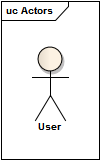
\includegraphics[scale=1]{../ea_files/generatedImages/Simulator/Actors.png}
			\caption{Actors of simulation tool.}
			\label{fig:actors}
		\end{figure}
		
		\begin{figure}[!hbtp]
			\centering
			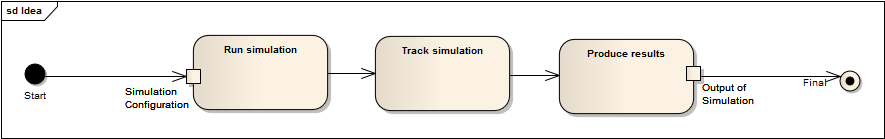
\includegraphics[width=\textwidth]{../ea_files/generatedImages/Simulator/Idea.png}
			\caption{Idea, happy path of a simulation.}
			\label{fig:idea}
		\end{figure}
	
		\begin{figure}[!hbtp]
			\centering
			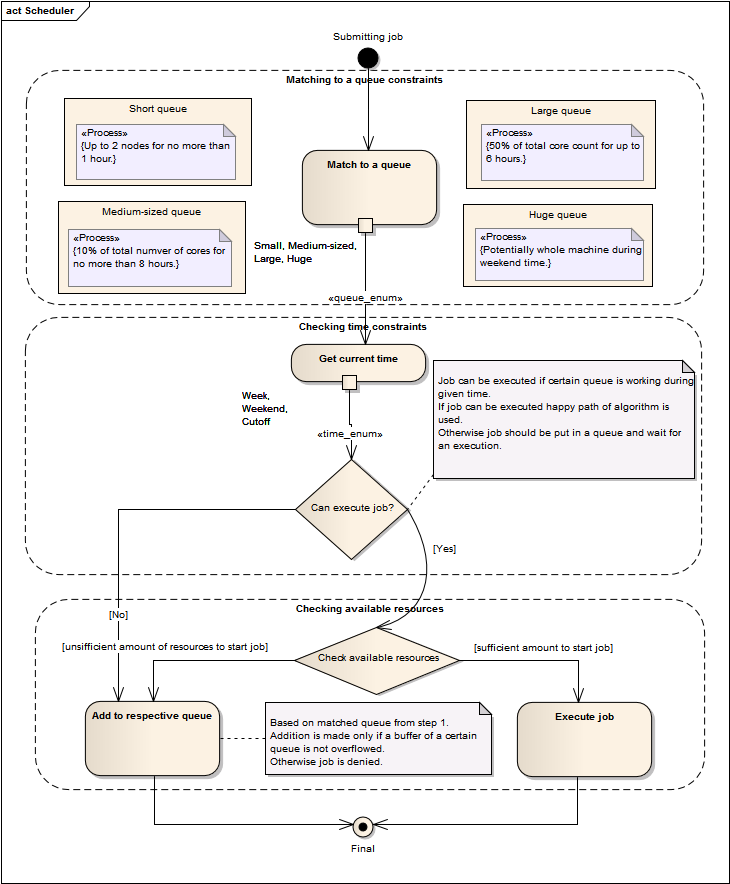
\includegraphics[width=\textwidth]{../ea_files/generatedImages/Simulator/Scheduler.png}
			\caption{Scheduling algorithm of a simulation tool.}
			\label{fig:scheduler}
		\end{figure}
	
		\begin{figure}[!hbtp]
			\centering
			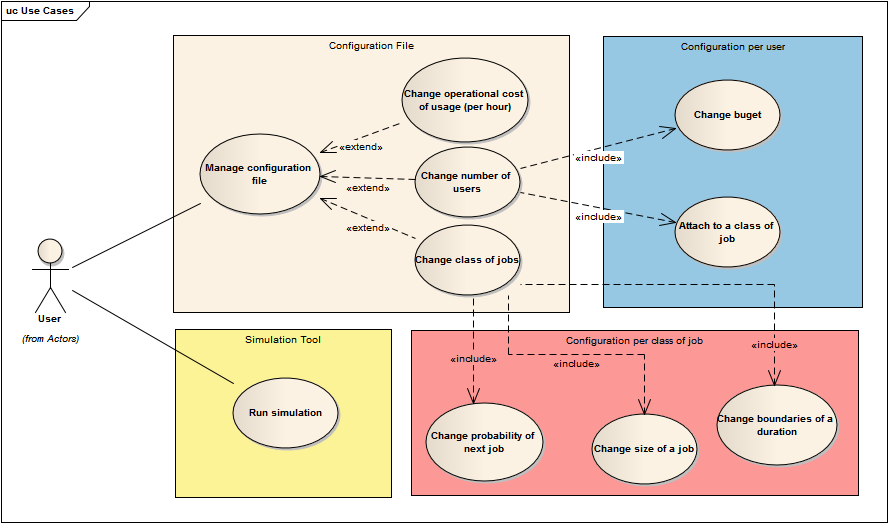
\includegraphics[height=\textwidth, angle=90]{../ea_files/generatedImages/Simulator/UseCases.png}
			\caption{Use cases for simulation software.}
			\label{fig:use-cases}
		\end{figure}
\end{appendices}